\section{Évolution de la vitesse avec la distance}

\subsection{Introduction}

Dès sa sortie du canon, un projectile est soumis à la résistance de l'air. Cette force s'oppose à son mouvement et provoque une diminution progressive de sa vitesse.

Contrairement à une intuition courante, cette diminution n'est pas linéaire. La décélération est généralement plus importante aux grandes vitesses puis diminue progressivement au fur et à mesure que le projectile ralentit.

L'étude de la vitesse résiduelle est fondamentale en balistique extérieure car elle influence directement :

\begin{itemize}
\item la portée ;
\item le temps de vol ;
\item la chute du projectile ;
\item la sensibilité au vent ;
\item l'énergie cinétique disponible à l'impact.
\end{itemize}

\subsection{Exemple de courbes de décélération}

La figure \ref{fig:vitesse_distance} présente trois profils de projectiles fictifs possédant des caractéristiques aérodynamiques différentes.

\begin{figure}[H]
\centering
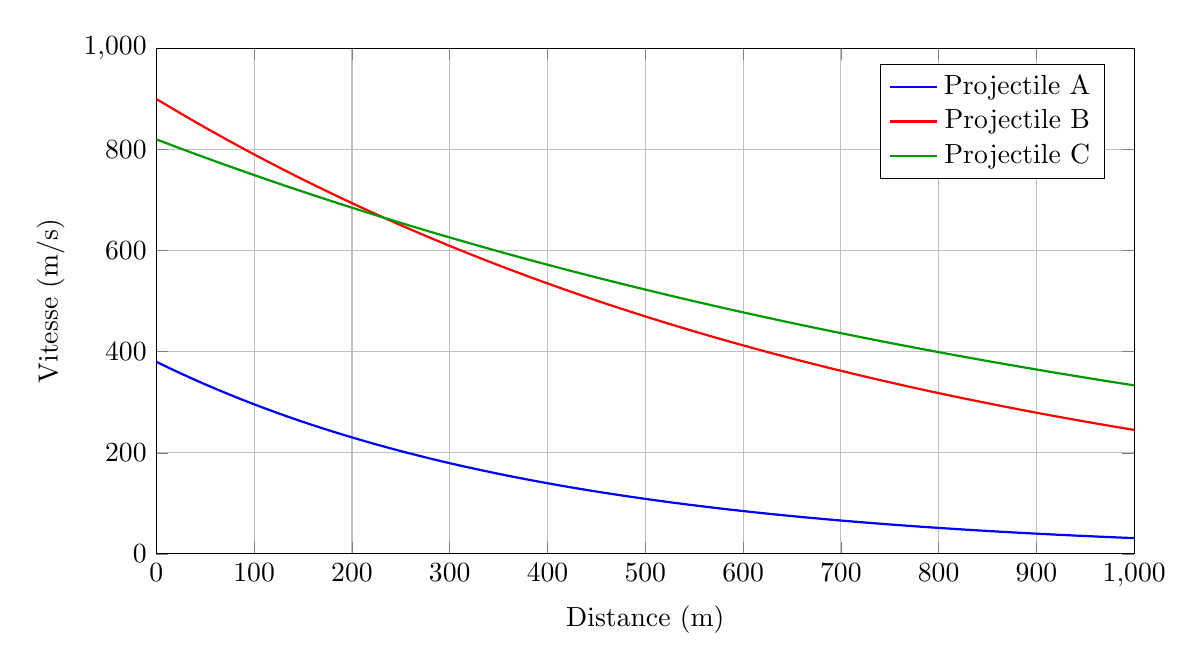
\begin{tikzpicture}

\begin{axis}[
    width=14cm,
    height=8cm,
    xlabel={Distance (m)},
    ylabel={Vitesse (m/s)},
    xmin=0,
    xmax=1000,
    ymin=0,
    ymax=1000,
    grid=major,
    legend pos=north east
]

\addplot[blue, thick, domain=0:1000,samples=200]
{380*exp(-0.0025*x)};
\addlegendentry{Projectile A}

\addplot[red, thick, domain=0:1000,samples=200]
{900*exp(-0.0013*x)};
\addlegendentry{Projectile B}

\addplot[green!60!black, thick, domain=0:1000,samples=200]
{820*exp(-0.0009*x)};
\addlegendentry{Projectile C}

\end{axis}

\end{tikzpicture}

\caption{Évolution qualitative de la vitesse en fonction de la distance}
\label{fig:vitesse_distance}

\end{figure}

Les courbes peuvent être reproduites dans Desmos à l'aide des équations suivantes :

\begin{align}
V_A(x) &= 380*e^{-0.0025x} \\
V_B(x) &= 900*e^{-0.0013x} \\
V_C(x) &= 820*e^{-0.0009x}
\end{align}

où :

\begin{itemize}
\item $V(x)$ représente la vitesse en m/s ;
\item $x$ représente la distance parcourue en mètres.
\end{itemize}

En considérant que :

\begin{equation}
V(x)=V_0\,e^{-kx}
\end{equation}

où :

\begin{itemize}
\item $V(x)$ représente la vitesse en m/s ;
\item $V0$ représente la vitesse initiale en m/s ;
\item $k$ représente le coefficient de décélération ;
\item $x$ représente la distance parcourue en mètres.
\end{itemize}


Cependant, il faut garder à l'esprit que ce modèle est une simplification pédagogique.

En balistique réelle, la vitesse ne suit pas exactement une exponentielle simple :

\begin{equation}
V(x)\neq\,V_0\,e^{-kx}
\end{equation}

car la traînée dépend notamment :

\begin{itemize}
\item de la vitesse instantanée ;
\item de la densité de l'air ;
\item du régime subsonique, transsonique ou supersonique ;
\item du coefficient balistique.
\end{itemize}

Les courbes réelles sont généralement plus complexes.

\subsection{Interprétation}

Le projectile A présente une perte de vitesse rapide. Sa trajectoire est fortement affectée par la gravité et le vent.

Le projectile B possède une vitesse initiale plus élevée et conserve son énergie sur une plus grande distance.

Le projectile C présente la meilleure conservation de vitesse. Sa décélération est plus faible grâce à de meilleures caractéristiques aérodynamiques.

\subsection{Lien avec l'énergie cinétique}

L'énergie cinétique est donnée par :

\begin{equation}
E_c=\frac{1}{2}mv^2
\end{equation}

Cette relation montre que l'énergie dépend du carré de la vitesse.

Ainsi, une perte modérée de vitesse entraîne une diminution importante de l'énergie cinétique disponible.

\subsection{Conséquences balistiques}

La diminution de la vitesse entraîne plusieurs effets :

\begin{enumerate}
\item augmentation du temps de vol ;
\item augmentation de la chute gravitationnelle ;
\item augmentation de la dérive due au vent ;
\item diminution de l'énergie cinétique ;
\item augmentation de la sensibilité aux perturbations extérieures.
\end{enumerate}

Pour cette raison, la conservation de la vitesse constitue l'un des paramètres les plus importants en balistique extérieure.

\subsection{Conclusion}

La vitesse d'un projectile décroît continuellement sous l'effet de la résistance de l'air. Cette perte de vitesse modifie simultanément la trajectoire, le temps de vol et l'énergie cinétique.

L'étude de la vitesse résiduelle constitue donc l'un des outils fondamentaux permettant de comprendre le comportement d'un projectile tout au long de son vol.

